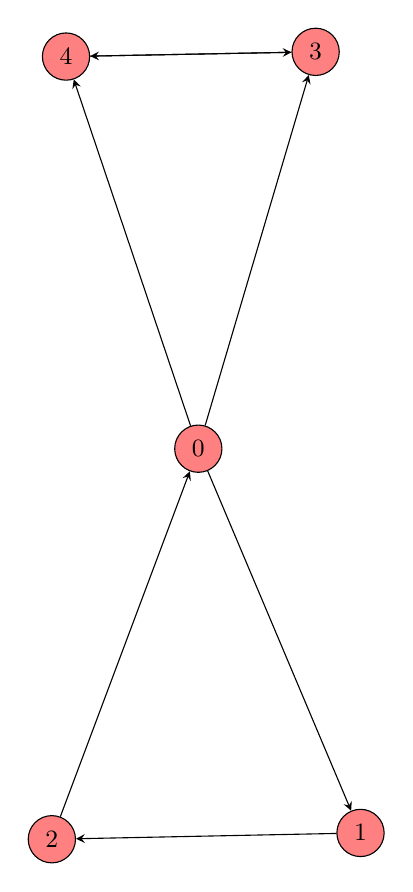
\begin{tikzpicture}[>=stealth, node distance=2cm, every loop/.style={min distance=10mm}]
\node[circle, draw=black, fill=red!50, inner sep=0pt, minimum size=6mm] (node0) at (1.86, 4.96) {\small 0};
\node[circle, draw=black, fill=red!50, inner sep=0pt, minimum size=6mm] (node1) at (3.92, 0.08) {\small 1};
\node[circle, draw=black, fill=red!50, inner sep=0pt, minimum size=6mm] (node2) at (0.00, 0.00) {\small 2};
\node[circle, draw=black, fill=red!50, inner sep=0pt, minimum size=6mm] (node3) at (3.35, 10.00) {\small 3};
\node[circle, draw=black, fill=red!50, inner sep=0pt, minimum size=6mm] (node4) at (0.18, 9.94) {\small 4};
\draw[->] (node0) -- (node1);
\draw[->] (node0) -- (node3);
\draw[->] (node0) -- (node4);
\draw[->] (node1) -- (node2);
\draw[->] (node2) -- (node0);
\draw[->] (node3) -- (node4);
\draw[->] (node4) -- (node3);
\end{tikzpicture}
